% !TeX spellcheck = en_US


\part{Getting started}
\label{part:GettingStarted}

\chapter{Overview}

\section{Introduction}

This part of the book will run the reader through the LedgerSMB using an example
startup company run by Jack: Example Inc, which starts its life as a computer parts
store for the business to business market.

Jack just completed incorporation of Example and is ready to start doing business.
Before starting his operation Jack decides to look for tooling to run his operation
efficiently.

The other chapters in this part of the book show you what steps Jack has to go through
to get LedgerSMB up and running for Example, as well as the steps he has to take to
keep LedgerSMB in good health.

Due to its success Example will grow, posing new challenges to LedgerSMB and we'll show
you how Jack can change the configuration to adapt to his growing business's needs.

Jack chooses to use a hosted LedgerSMB, so he doesn't need to concern himself with the
technical details of getting the application up and running. Instead he can start by setting
up the company database immediately.

In \charef{cha:CompanyCreation} and \charef{cha:the-first-login} Jack goes through the
steps of setting up a basic company. The chapters after that may not apply to every
business. \charef{cha:building-up-stock}, \charef{cha:ramping-up-to-the-first-sale} and
\charef{cha:shipping-sales} apply to businesses dealing with physical goods: buying,
selling and shipping. \charef{cha:invoicing} discusses how to handle invoicing from LedgerSMB.
\charef{cha:customer-payments}, \charef{cha:vendor-payments} and \charef{cha:monitoring-arrears}
discuss how to manage accounts receivable and payable including arrears monitoring.

Not all chapters may be relevant to the reader, e.g. when he or she is starting up or
running a services company in which case the chapter ``Building up stock'' doesn't apply.
Chapters can be skipped based on relevance both to the type of business and its growth
phase.

@@@ more chapters??

\section{LedgerSMB, because...}

@@@ This seems to be a full overlap with \charef{cha:Advocacy}.

Jack finds several tools which suit his requirements to some extent or another.
After evaluation of his options he decides to use LedgerSMB for the following reasons:

\begin{itemize}
\item Centralized data storage
\item Actively developed
\item Development team with security focus
\item Access to the application requires only a web browser
\item Integrated sales, shipping, invoicing, purchasing and accounting
\item Open source solution, so no vendor lock in
\item The roadmap appeals to him, because it has web services payrolling on it
\item There are multiple vendors offering commercial support, including hosted options
\item The developers envision building a platform out of it: creating the building blocks
required to build a company on
\end{itemize}

He'll be running LedgerSMB using the domain he acquired for his business:
\url{http://example.com/}.

\chapter{Creating a company}
\label{cha:CompanyCreation}

\section{Using setup.pl}

LedgerSMB comes with a tool called 'setup.pl'. It's the beginning of a web-based
database administration interface to LedgerSMB. This tool can be used to create
company databases as well as backups of existing ones. There's also a command line based
Unix-only setup tool - this tool is covered in the next section.

Please note that while executing the steps described in this section, it may take a while
for the next screen to appear after clicking on each button: Some buttons involve
a large amount of processing on the server before the next screen can be presented.

\subsection{Step 1: setup.pl login}

Jack installed LedgerSMB using the default installation instructions, which means
that the url for his setup.pl is \url{https://example.com/ledgersmb/setup.pl}.
\figref{fig:setup-step1} shows the login screen for the tool.

\begin{quotation}
Please note that you can't be logged into the administration tool (setup.pl) and the webapp
through the same browser at the same time in this version of LedgerSMB - due to technicalities.
\end{quotation}

The login screen shows three fields: (a) a user, (b) a password and (c) a database name.

The user name you use to log in needs to be a PostgreSQL super user: a user you can use
to log into the database using the ``psql'' command as well.

The password must be the same as the one used to log in from the command line using the
``psql'' tool or the password you used upon creation using the ``createdb'' tool. Both
``psql'' and ``createdb'' are PostgreSQL tools (not LedgerSMB tools).

The third field is the name of the database to be created, which is the same as the
name of the company to be logged into later on through the login page shown in \figref{fig:login-screen}. The next paragraph discusses this field and its meaning more
in-depth.

\begin{figure}[h]
\centering
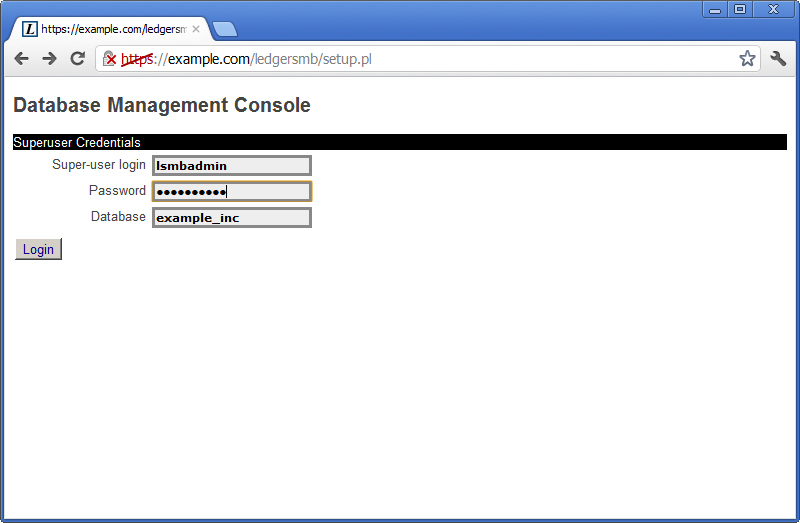
\includegraphics[width=7cm]{dmc-create-step1.png}
\caption{setup.pl login screen}
\label{fig:setup-step1}
\end{figure}

\subsection{Step 2: Company creation}

When creating a company database, there are a few things that are of importance:

\begin{itemize}
\item The name of the database is the same as the name used at login time and hence
   will be used by all users - a choice of a suitable, recognizable value is important
\item The name of the database entered (and hence the company name) is case-sensitive
\item The name can't be more than 63 characters long
% \item ### others?
\end{itemize}

After choosing ``example\_inc'' as his company name, Jack clicks the Login button at which
time the screen from \figref{fig:setup-step2} shows up. The screen says the database doesn't
yet exist and offers its creation. The backup buttons being offered are not useful at this
stage - they have value if the database exists and setup.pl is being used to upgrade
the database; one of its other functionalities.

\begin{figure}[h]
\centering
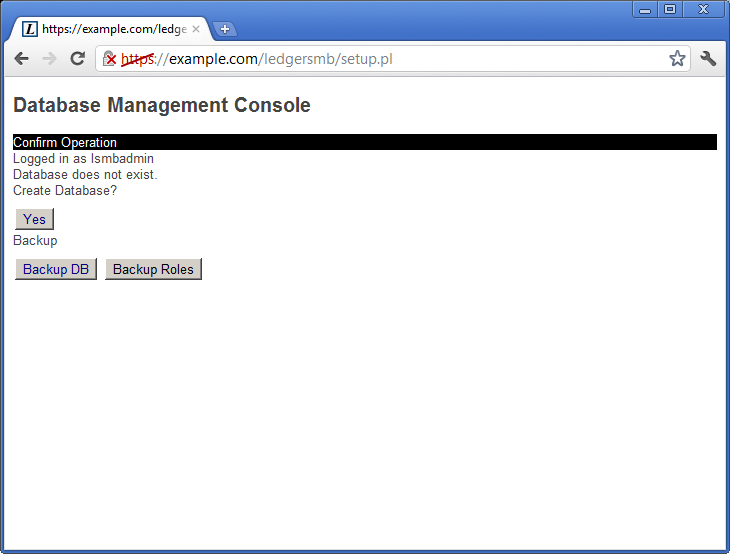
\includegraphics[width=7cm]{dmc-create-step2.png}
\caption{setup.pl company creation screen}
\label{fig:setup-step2}
\end{figure}

Jack clicks ``Yes'' to create the database and load it with LedgerSMB's database
schema, authorization rules and stored
procedures\footnote{Parts of the program inside the database.}. It may
take a while (30 seconds or more) for the next screen to appear\footnote{Note 
that during the creation of the database, logs are kept so that if there are
errors these can be reviewed either by the person installing the software or by
support personnel.  On Linux/Unix systems these are stored, by default, in
/tmp/ledgersmb/ and named dblog, dblog\_stderr and dblog\_stdout.}.

\subsection{Step 3: Selection of a Chart of Accounts}

LedgerSMB comes with numerous predefined charts of accounts. These have been grouped
per country making the selection of a chart a two-step procedure. setup.pl allows for
users wanting to define their own charts by offering a ``Skip'' button. This button
skips the process of loading a chart.

\begin{quote}
Note that you need to define a chart of accounts before you can meaningfully do anything
inside LedgerSMB. If you don't load a pre-defined one you'll need to create or import your
own later.
\end{quote}

\figref{fig:setup-step3} shows the first screen in the chart of accounts selection procedure.
In this screen you select the country for which you want to use the chart of accounts. Note
that charts of accounts are highly country dependent and you may want to consult
an accountant if no default chart of accounts is included for your country.

As Jack runs his company in the US, that's what he selects.

\begin{figure}[h]
\centering
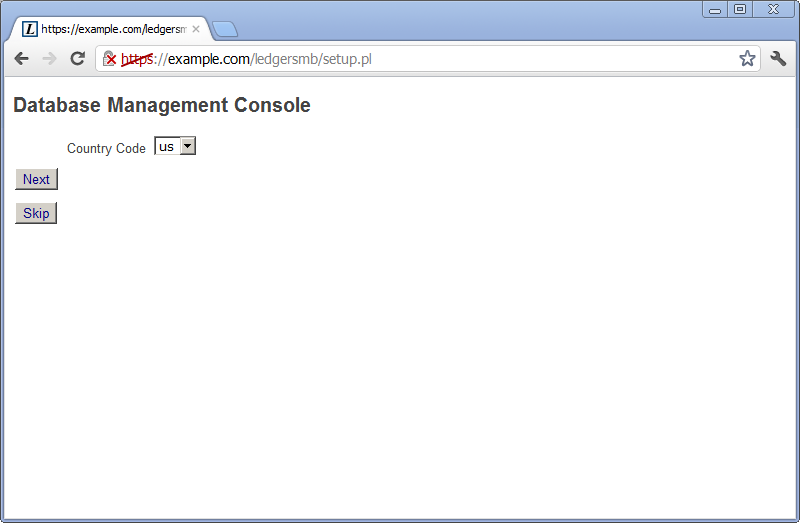
\includegraphics[width=7cm]{dmc-create-step3.png}
\caption{Chart of accounts - Country selection}
\label{fig:setup-step3}
\end{figure}

\figref{fig:setup-step4} shows the second screen in the chart of accounts selection procedure.
The drop down contains a list of all charts of accounts defined for the selected country.

Jack selects the General.sql chart of accounts: that will leave him enough room to specialize
the setup later if he has to, but for the time being offers a broadly useable setup.

\begin{figure}[h]
\centering
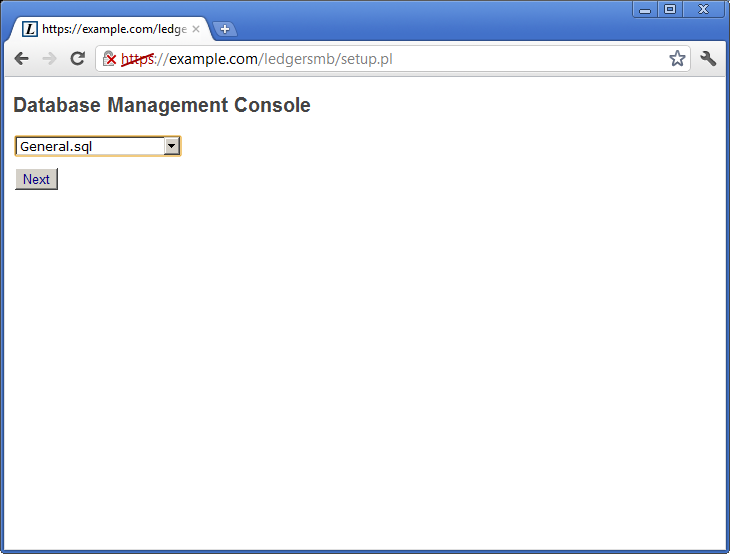
\includegraphics[width=7cm]{dmc-create-step4.png}
\caption{Chart of accounts - Chart selection}
\label{fig:setup-step4}
\end{figure}


\subsection{Step 4: First user}

In the last paragraph the technical part of the company creation procedure was completed.
However, it's not possible to log in to the company yet. This paragraph describes how to
create a first user.
\figref{fig:setup-step5} shows the user creation screen. The fields in this screen have
the same meaning as those discussed as part of user management in \secref{sec:user-creation}.

\begin{figure}[h]
\centering
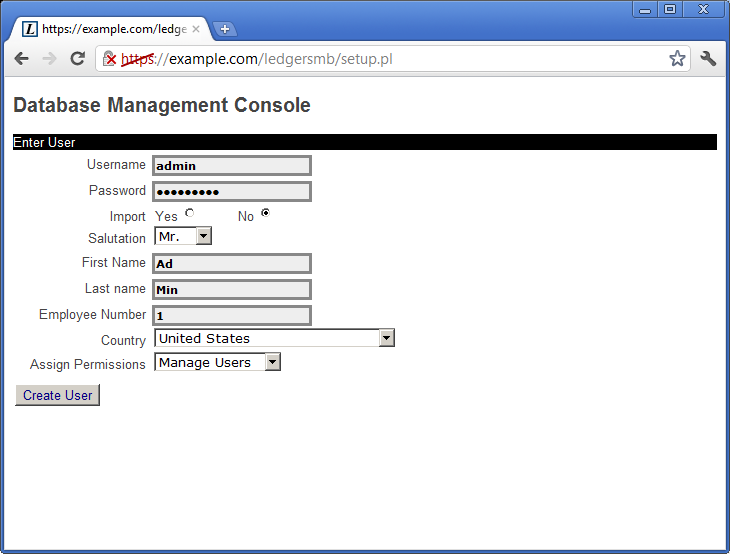
\includegraphics[width=7cm]{dmc-create-step5.png}
\caption{setup.pl initial user creation screen}
\label{fig:setup-step5}
\end{figure}

Jack chooses to create an administrative user called \texttt{admin} who will be authorized
to do everything in the application. Later on he will also create a user \texttt{jack}
who will be authorized to do everything but changing the configuration and doing application administration.
He'll use the latter user to log in for day to day operations. This will help him prevent
changing things by accident.

Note that none of the fields in this screen are optional. If the name of the user being created
isn't already used with other companies, leave the \texttt{Import} option set to \texttt{No},
otherwise please read the chapter on user creation mentioned above.

\begin{quotation}
Note: The password you enter here is a temporary one which will remain in effect for 24
hours only. Be sure to execute the steps in \secref{sec:steps-to-the-first-login} before
these 24 hours elapse, because the user will be disabled after that.
\end{quotation}

The setup.pl program offers the user to be created to be one of two types:

\begin{itemize}
\item Manage Users
\item All Permissions
\end{itemize}

Jack's choice for a fully authorized \texttt{admin} user leads him to select the
\texttt{All permissions} option.

\begin{figure}[h]
\centering
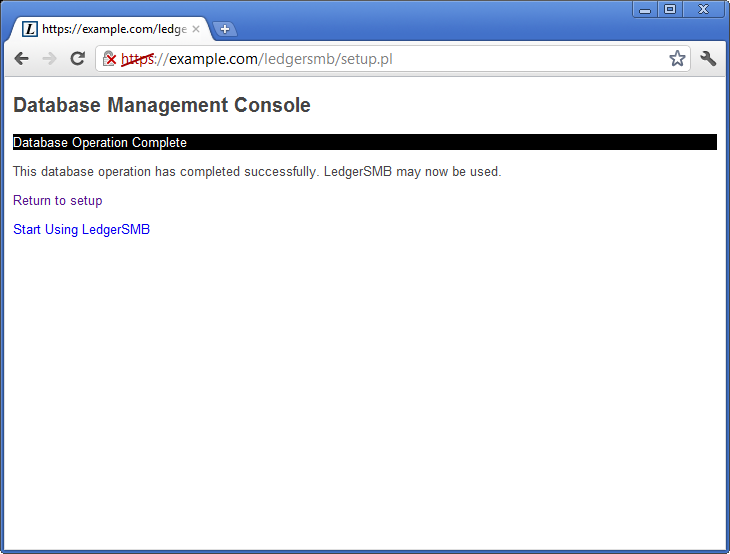
\includegraphics[width=7cm]{dmc-create-step6.png}
\caption{setup.pl successful completion screen}
\label{fig:setup-step6}
\end{figure}

Jack succeeded to correctly create his company database. His story continues in
the next chapter ``The first login''.

\section{Using prepare-company-database.sh}

To be done.


\chapter{The first login}
\label{cha:the-first-login}

\section{Introduction}

After the company has been created by executing the procedure described in the last
chapter it is still an empty shell which needs to be populated. The correct data
needs to be entered for things like bank accounts and company contact data to be used
on invoices.

These steps have to be completed before LedgerSMB can be used meaningfully: these
settings have to be present for many workflows. A major reason is that with LedgerSMB
- as most ERP systems - financial
consequences of events in many workflows are directly reflected in the company's books.
Some accounting related settings have to be completed before LedgerSMB can do so.

This chapter documents the steps to this configuration. It assumes you've did not skip
loading a chart of accounts in \charef{cha:CompanyCreation} or that - if you did -
imported your own. Whatever your method, a chart of accounts should be available.

\section{Steps to the first login}
\label{sec:steps-to-the-first-login}

After Jack finishes the last chapter, he clicks the \texttt{Start using LedgerSMB} link
shown in \figref{fig:setup-step6}.


\subsection{Login screen}

\begin{figure}[h]
\centering
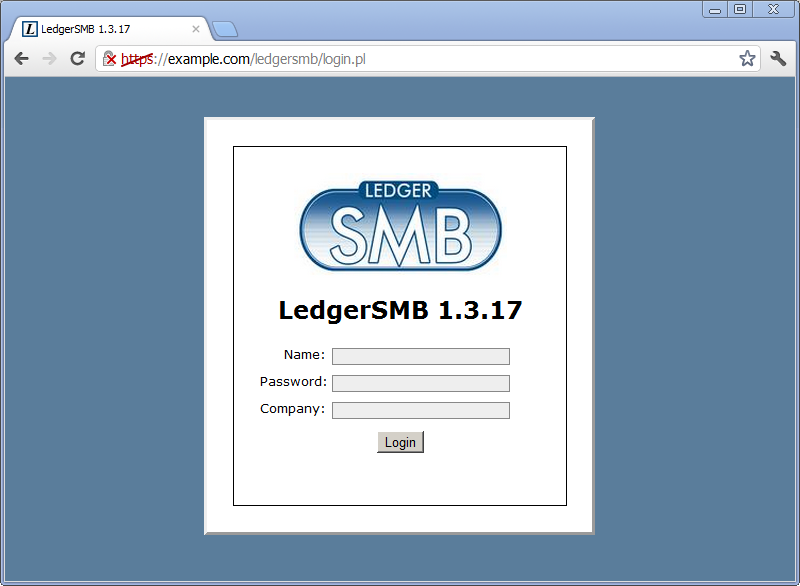
\includegraphics[width=7cm]{dmc-create-final.png}
\caption{login.pl opening screen}
\label{fig:login-screen}
\end{figure}

The login screen shows three fields which need to be filled out as follows:

\begin{description}
\item[Name] The user name created during database setup; Jack uses \texttt{admin}
\item[Password] The password - in this case for Jack's \texttt{admin} user
\item[Company] The name of the database created; Jack uses \texttt{example\_inc}
\end{description}

\subsection{Selecting a password}

After successful login, the system shows the user preferences screen as depicted in
\figref{fig:first-login-password} to facilitate the required password change. The
initial password has a 24-hour validity limit to prevent unused user accounts from posing
a security risk.

The password Jack chooses may be either the same as the one he used before.
Not clicking the \texttt{Save} button means the password remains unchanged and the
24-hour limit remains in effect.

\begin{figure}[h]
\centering
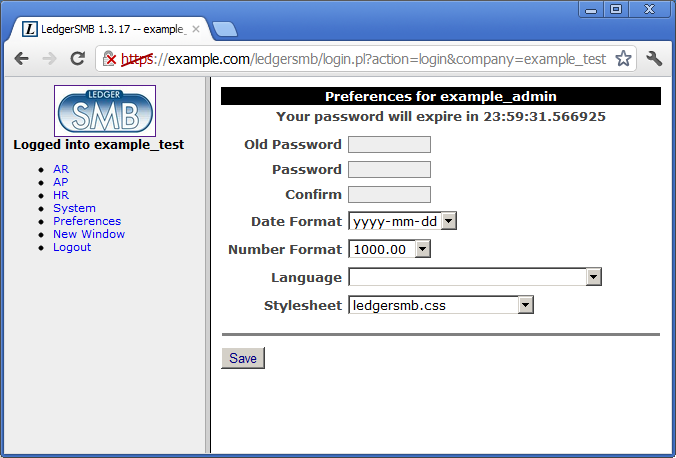
\includegraphics[width=7cm]{first-login-password.png}
\caption{First login password selection}
\label{fig:first-login-password}
\end{figure}

The new password has a validity of determined by the \texttt{Password Duration} setting
from the System $\rightarrow$ Defaults screen. User management is discussed is detail in \charef{cha:user-management}.

The password reset dialog won't show on subsequent logins until one week
before expiry. Login will be denied to users with expired passwords; they can request
password resets through user admins.


\section{Setting up a bank account or credit card}
\label{sec:setup-bank-account}

As part of the start up activities of his company, Jack comes to an agreement with the
bank for three products:

\begin{itemize}
\item A current account with number ``C54769''
\item Deposit account with number ``D54990''
\item Credit card with a number ending with ``.7734''
\end{itemize}

Most accounting systems - LedgerSMB included - use separate GL accounts to represent
each bank account. This allows easy reconciliation of the ending balance on the bank
account with the balance in the books.

Knowing this, Jack looks up the example bank account from his preconfigured US chart of
accounts using the System $\rightarrow$ Chart of Accounts $\rightarrow$ List Accounts menu as
shown in \figref{fig:bank-setup1}.

\begin{figure}[h]
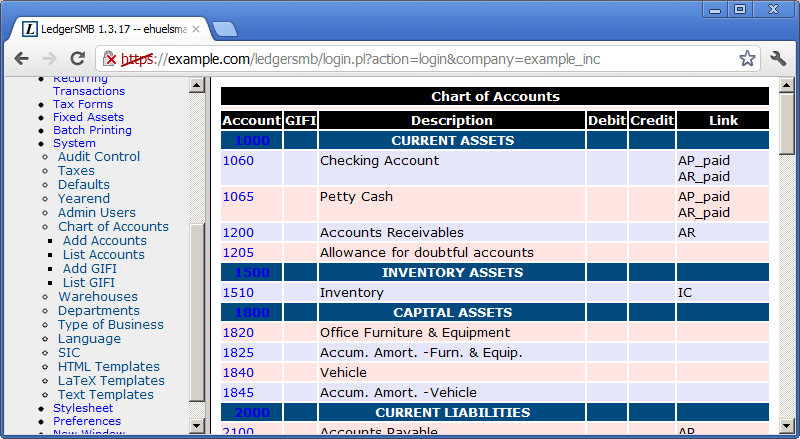
\includegraphics[width=\linewidth]{setup-bank-account1.png}
\caption{Bank account setup - menu items}
\label{fig:bank-setup1}
\end{figure}



\begin{enumerate}
\item Renames the original account 1060 ``Checking account'' into ``Checking account C54769''
\item Click ``Save''
\item Open the 1060 account again
\label{itm:bank-setup-steps-start}
\item Change the number to 1061
\item Change the description to ``Cash deposit account D54990''
\item Click ``Save as''
\label{itm:bank-setup-steps-end}
\end{enumerate}

Then Jack repeats the steps \ref{itm:bank-setup-steps-start} to \ref{itm:bank-setup-steps-end}
for the credit card with the account number 1062 and description ``Credit card xxxx.xxxx.7734'' to set
up the credit card. \figref{fig:bank-setup2} shows the screen in which to enter the account
details. \secref{sec:AccountOptions} discusses the options in detail - for now using the
settings as configured for the sample checking account will do.

\begin{figure}[h]
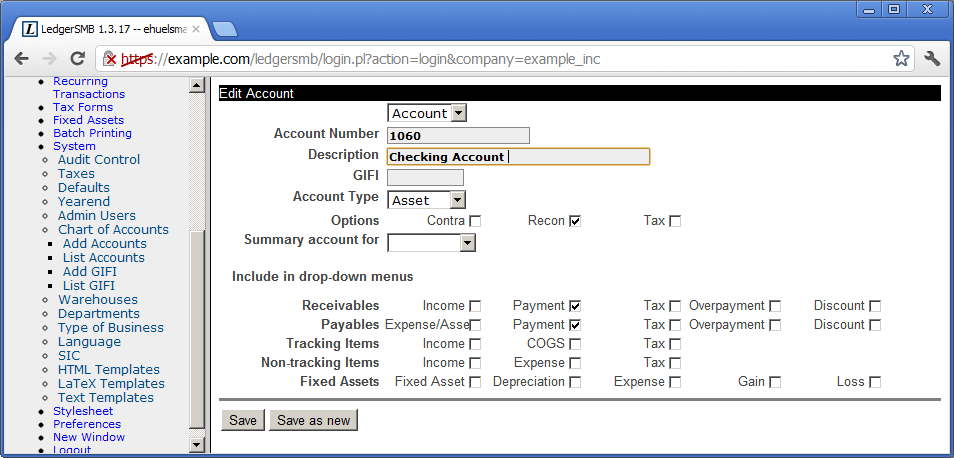
\includegraphics[width=\linewidth]{setup-bank-account2.png}
\caption{Bank account setup - account setup screen}
\label{fig:bank-setup2}
\end{figure}


\section{Checking and adjusting the chart of accounts}
\label{sec:checking-the-coa}

First and foremost the chart of accounts serves to register income, expenses,
assets and liabilities in categories which support financial decision making or
regulatory requirements. When checking his chart of accounts, this is the first
thing Jack checks for.

Many business events in LedgerSMB trigger the creation of financial transactions.
If the configuration required for these transactions to be created isn't in place,
users won't be able to complete their workflows. 

\subsection{Accounts list}

Jack wants to make sure his chart of accounts fits his purposes. To perform these
checks Jack goes into the System $\rightarrow$ Chart of Accounts $\rightarrow$
List Accounts page. For now, he finds
the ledger to be in order. Although the single Sales account stands out a bit against
the numerous expense accounts, it turns out that there is also a single Purchases
account on which all the expenses for parts purchases are going to be booked.

He decides that if this isn't enough, he can add accounts later.
\footnote{Note that Jack will discover in \secref{sec:defining-vendors} that
he does indeed need to create additional accounts to support sales and
purchase discounts.}

\subsection{Technical accounts identified by Links}

For LedgerSMB to operate correctly, a number of accounts have to be configured for
their specific purpose. He continues on the same screen as the previous section. His
checks concern the values in the \texttt{Link} column of the screen. These values have
to be present:

\begin{longtable}{ lp{8cm} }
Purpose & Description \\ \hline
\endhead
AR  & The summary account for accounts receivables; most example charts of accounts have one. \\
AR\_overpayment & Receivables overpayments; if a customer pays too much or gets a credit
                  invoice for an invoice already paid, this is where his credit gets
                  recorded if it's not refunded immediately \\
AR\_discount & Sales discounts; if a customer pays within the specified terms, a discount
                  is applied.
                  In order to monitor effectiveness of the discount offered, one probably
                  wants it posted on its own account. \\
AP  & Same as AR, except for payables. \\
AP\_overpayment  & Same as AR\_overpayment, except that this registers credits others owe you \\
AP\_discount &  Same as AR\_discount, except that it applies to payables \\
IC  & Summary account for inventory; this account doesn't apply to companies which sell
      services only. \\

\caption{List of special purpose account types by link}
\label{tbl:special-purpose-account-types-links}
\end{longtable}


Jack's chart (the US General.sql standard chart) misses the AR and AP\_overpayment links as
well as the overpayment accounts. He'll need to create them by going to the Add Accounts under
the same submenu as the List Accounts option. The table below shows the settings required for
the account types listed in Table \ref{tbl:special-purpose-account-types-links}.

\begin{longtable}{lll}
Purpose & Account type & Overpayment checkmark line \\ \hline
\endhead
AR & Asset &  \\
\textit{AR\_overpayment} & \textit{Liability} & \textit{Receivables} \\
AR\_discount & Income (Contra) &  \\
AP & Liability &  \\
\textit{AP\_overpayment} & \textit{Asset} & \textit{Payables} \\
AP\_discount & Expense (Contra) & \\
IC & Asset &  \\
\caption{Special purpose account configuration summary}
\label{tbl:special-purpose-account-config-summary}
\end{longtable}

Jack creates two accounts, one for each line marked in italics in Table \ref{tbl:special-purpose-account-config-summary}:
\begin{itemize}
\item [1202] Advance payments
\item [2105] Advance receipts
\end{itemize}


\subsection{Technical accounts from System Defaults}
\label{subsec:technical-accounts-system-defaults}

Two special purpose accounts are currently not assigned their special purpose through
the Links column in the Chart of Accounts menu. Instead, their special purpose is indicated
in the defaults screen as discussed in \secref{sec:setting-up-system-defaults}.

Each chart of accounts should have
\begin{itemize}
\item a foreign exchange gain account in the Income part
\item a foreign exchange loss account in the Expense part
\end{itemize}

This restriction applies even for companies which don't expect to be using foreign currencies
since the accounts \textbf{have} to be selected in the defaults screen: there's no option
to leave them blank.

\section{Checking sales tax (VAT) rates}

First off, Jack asserts that a sales tax account has been provisioned. He finds it
in the Current Liabilities section of his chart of accounts. In his jurisdiction there
is only one sales tax rate applicable at any one time, which means this single account
will suit his needs just fine. If he had been in a jurisdiction with multiple tax rates
applicable, e.g. different rates for different types of goods, he would have been
required to create more accounts.

The procedure to create more sales tax accounts is the same as the one used in
\secref{sec:setup-bank-account}, with the notable difference that this time the base account
to be used is the sales tax account.

With the accounts in place, the tax rates have to be checked and possibly adjusted.
To do so, go to the System $\rightarrow$ Taxes page as shown in \figref{fig:setup-tax-rates}.

\begin{figure}[h]
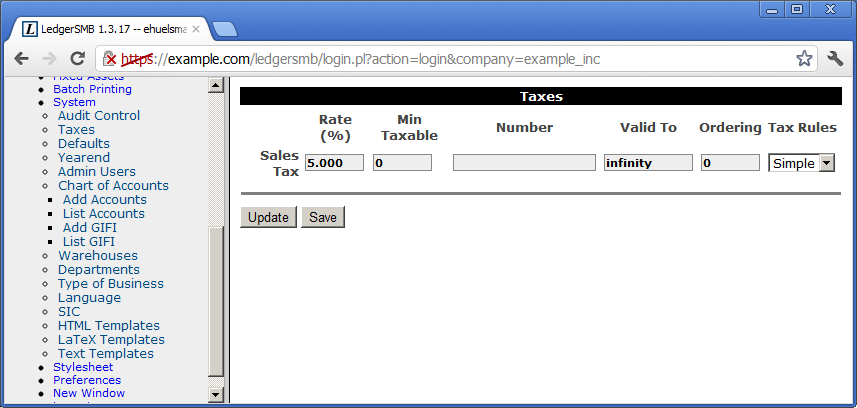
\includegraphics[width=\linewidth]{setup-tax-rates.png}
\caption{Tax rate adjustment screen}
\label{fig:setup-tax-rates}
\end{figure}

The rate shown (5\%) is exactly what Jack needs. The procedure to set rates is a bit
long to describe and hence has its own chapter. Please refer to \charef{cha:Taxes} for
details on how to change taxes.

\section{Setting up the system defaults}
\label{sec:setting-up-system-defaults}

With the password renewal out of the way, Jack can start to set up the company for first
use. To do so, Jack selects the System $\rightarrow$ Defaults menu item.

A more elaborate description of the parameters in this screen is provided in subsection
\ref{subsec:Defaults}. However, when setting up a new company, it's probably good enough
to fill out these parameters (and thus skip the rest):

\begin{itemize}
\item Business number (e.g. Chamber of commerce number) [12345]
\item Default language [English]
\item Default accounts (Inventory, Expense, Income) [1510 Inventory / 4010 Sales / 5010 Purchases]
\item Foreign exchange result accounts (Foreign exchange gain/ loss) [4450 Gain / 5810 Loss]
\item Default country [US]
\item Templates directory [demo]
\item Currencies [USD:CAD]
\item Password Duration [180]
\item Default Email From [info@example.com]
\item Company Name [Example Inc.]
\item Company Address [215 Example street - Whereitsat]
\item Company Phone [555 836 22 55]
\item Company Fax (optional) [N/A]
\end{itemize}

Jack enters the values mentioned between the square brackets in the list above.



\chapter{Building up stock}
\label{cha:building-up-stock}

\section{Overview}

In this chapter Jack goes through the process of setting up LedgerSMB for his
trade activities in computer parts, which includes deciding which parts he wants to
resell. From there on he goes to contact a vendor to request a quotation, convert that
to an order and receive goods into inventory and invoices into accounts payable.

To prepare LedgerSMB for his parts sales and purchases, Jack needs to configure Parts.
The system records inventory for parts and assemblies. Jack won't use them for his
business. There's more on assemblies in @@@.

Once set up, Jack is ready to execute the ordering process. Even though the process
is described here from a purchasing perspective sales work the same way with the roles
reversed (Jack will act as a vendor in the sales process).

To start his purchase, Jack creates a \gls{rfq} document which
he sends one or multiple vendors to let them know he's interested in their products.

The vendor responds to Jack's request by issuing a Quotation. From a legal perspective
a quotation is a document which promises to deliver the requested goods or services at a
certain rate - subject to conditions specifically mentioned. If Jack accepts the quotation
and meets the conditions, the vendor is obligated to deliver.

In response to the quotation, Jack will place an order with the vendor to indicate
acceptance quotation (or he can let the
it expire). When he places the order, that legally means he agrees to the terms
and conditions in the quotation. If the vendor delivers the goods or services as per the
order, Jack has accepted the legal obligation to pay.

The vendor responds to the order by shipping the goods and services as well
as sending an invoice. The invoice legally means the vendor considers to have a claim on the assets
of Jack's company. Jack creates a vendor invoice in his system to record the claim on his
company by the vendor and the vendor creates a sales invoice in their system to do the same.

As a result of the above it's considered bad practice to delete or change invoices once
created. The accepted process to adjust invoices is to generate a debit invoice (for purchases)
or a credit invoice (for sales) to ``undo'' the effects of the invoice and letting the other party
know about it. Then a new invoice can be generated with the appropriate content. However,
when the order process is correctly followed from order to invoice chances of sending the wrong
invoice are greatly reduced.

\section{Defining parts}

Jack needs to enter a large number of items he'll be offering in his new shop. He starts out
with the easy ones: the ones which will be sold as single items.

\subsection{Single items}

Jack chooses a 5TB hard drive by Samsung to be entered into the system as the first item.
To do so, he goes to the {\tt Goods and Services $\rightarrow$ Add part} page from the menu
as shown in @@@ (figure to be inserted).

Based on his reading from \secref{sec:DefinitionOfParts}, Jack decides to enter the hard
drive with the following data:

\begin{tabular}{ll}
Number & SAM5TB \\
Description & Samsung Hard drive 5TB / 7200rpm \\
Inventory account & 1510 - Inventory\\
Income account & 4010 - Sales\\
COGS account & 5010 - Purchases\\
Sell price & 75.00
\end{tabular}

He decides not to include make/model information, drawings or images yet and since
he hasn't entered vendors or customers in his system yet, he decides to leave
those sections blank as well.

\subsection{Combining single-item and ``multi-item pre-packaged'' sales}

After having finished setting up the easy parts, Jack now wants to enter
the memory modules he's going to sell. The problem is that they usually go in pairs,
since that's what the systems consuming them need. However, he expects them to be sold
as single items as well and he wants to be able to set a separate price for those occasions.

From his reading of \secref{subsec:parts-vs-assemblies-for-package-sales}, it should be
possible to support this scenario with a small work around\footnote{It's planned to directly
support this use-case in some version higher than 1.3}. From the two solutions available,
he chooses option (b): to create a part and an assembly and regularly restock the assembly
to 0 (zero) in order to remove the stock from the single item.

\section{Defining part groups}

As Jack continues to enter more parts into the system, he wonders how he's going to
look up the parts efficiently later on. Returning his reading to \secref{sec:DefinitionOfParts},
he understands that 'part groups' are the solution to that problem. He decides to create
the following list of part groups:

\begin{itemize}
\item Storage
\item Monitors
\item Input devices
\item Printers and MFPs
\end{itemize}

After creating these part groups, the ``Group'' drop down appears on the parts entry screen,
allowing him to assign each of his parts to one of these groups.

Since he doesn't expect to be running more than one or two types of CPUs, he decides
not to create a separate group for those and leaves these two parts unassigned.

\section{Defining vendors}
\label{sec:defining-vendors}

Jack selects ``ABC Parts'' to purchase the inventory he needs to run his company. In
order to start buying inventory, ABC Parts needs to be entered as a Vendor to LedgerSMB.

Using the work flow detailed in \secref{sec:creating-customers-and-vendors} Jack starts to do so by going through the menu \menupath{AP $\rightarrow$ Vendors $\rightarrow$ Add Vendor}.
 He fills out the Company creation form by clicking the {\tt Generate control code}
button and adding the data as shown in \figref{fig:vendor-create-1}.

\begin{figure}[h]
\centering
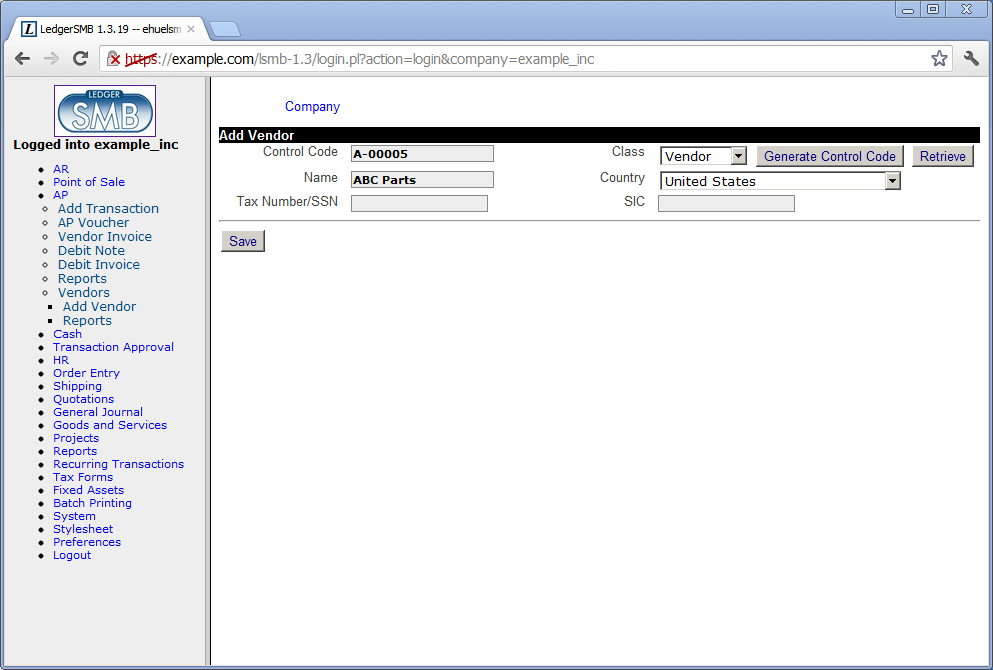
\includegraphics[width=7cm]{bus-vendor-create-2.png}
\caption{Company entry screen}
\label{fig:vendor-create-1}
\end{figure}

After saving the company data, Jack is presented the account data screen which he fills out
as shown in \figref{fig:vendor-create-2}.

\begin{figure}[h]
\centering
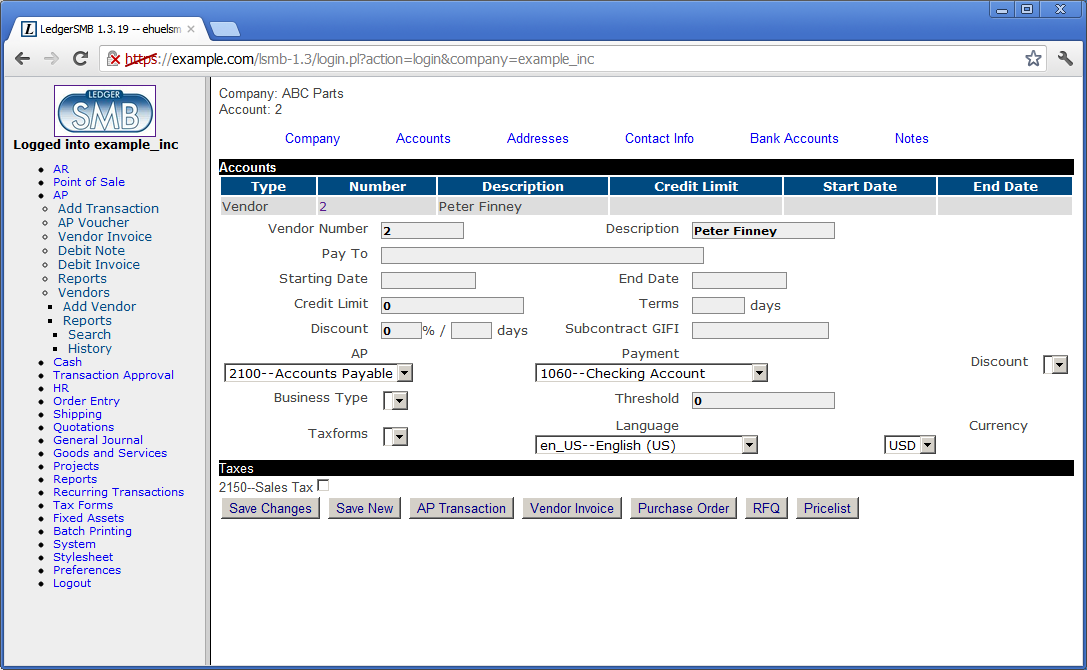
\includegraphics[width=7cm]{bus-vendor-create-3.png}
\caption{Vendor account screen}
\label{fig:vendor-create-2}
\end{figure}

When he's done filling out and saving the form,
he notices the empty ``Discount'' drop down. Reading more about account configuration
check marks in \secref{subsec:AR-AP-checkmarks} and going back to the checks on his
chart of accounts (\secref{sec:checking-the-coa}), he finds he's missing the purchase and
sales discount accounts. He adds two accounts as listed in \tabref{tbl:special-purpose-account-config-summary}:

\begin{itemize}
\item [4020] Sales discount
\item [5020] Purchase discount
\end{itemize}

After which the page looks like \figref{fig:vendor-create-3}.

\begin{figure}[h]
\centering
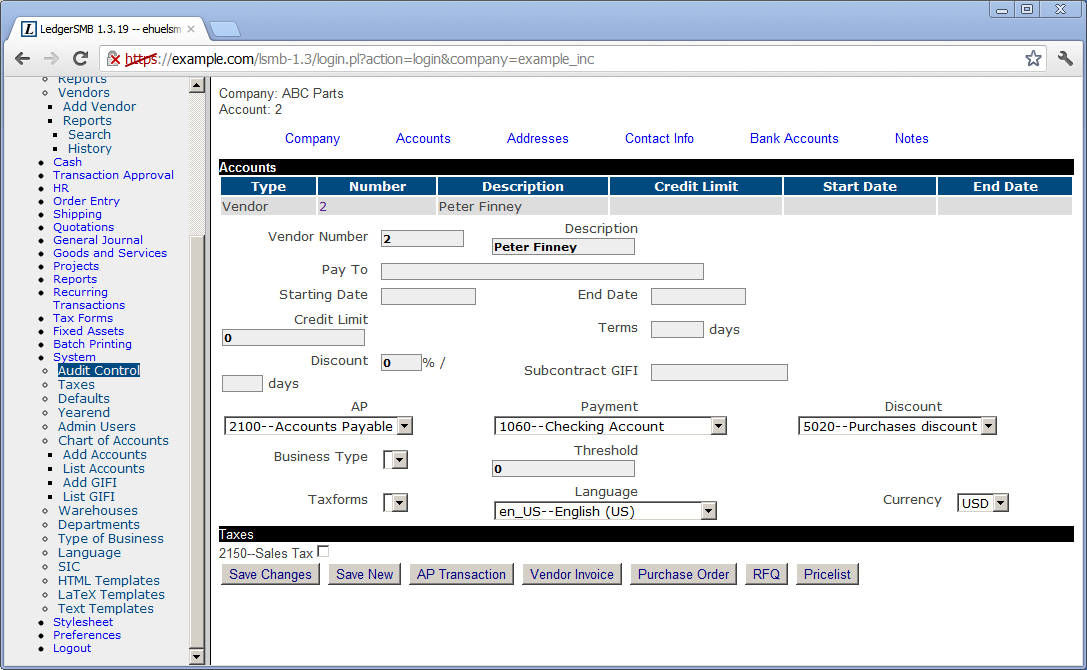
\includegraphics[width=7cm]{bus-vendor-create-4.png}
\caption{Vendor account screen - with purchase discount account}
\label{fig:vendor-create-3}
\end{figure}

Note the top-left corner stating ``Company: ABC Parts'' and ``Account: 2''. The information
entered on the ``Addresses'', ``Contact Info'' and ``Bank Accounts'' tabs will be attached
to the account listed, i.e. account number 2 in this case.

The reader is referred to \secref{sec:creating-customers-and-vendors} for a more in-depth
description of the vendor data screens.

\section{Requesting quotations}

After Jack finishes setting up the parts and vendor information, he decides to use LedgerSMB to draw
up a list of items he wants to order from this company. To do so he follows the menu path
\menupath{Quotations $\rightarrow$ RFQ} which opens up a screen (shown
in \figref{fig:rfq-entry-screen}) for entering a new \gls{rfq} .

\begin{figure}[h]
\centering
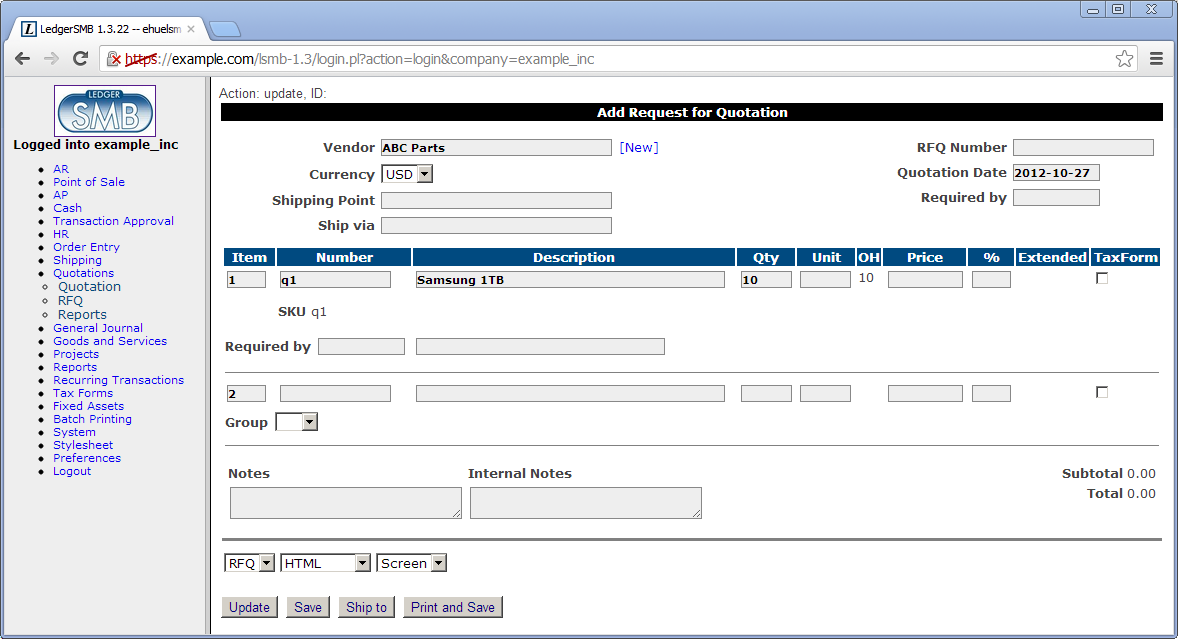
\includegraphics[width=7cm]{rfq-entry-screen.png}
\caption{RFQ entry screen}
\label{fig:bus-rfq-entry-screen}
\end{figure}

\begin{quotation}
\textbf{Remark} Note that the \gls{rfq} entry screen contains prices; this is misleading
at least: the printed output to be sent to the vendor does not. The fact that this screen
allows entry of prices could be considered a bug.
\end{quotation}

After filling out the form in accordance with the description in \secref{sec:creating-quotations},
Jack expedites his \gls{rfq} to his vendor through e-mail by clicking the ``E-mail'' button and
following the instructions \secref{subsec:sending-quotation-by-email}

\section{Following up on a quotation}

Jack's vendor (ABC Parts) sends him a quotation in response to his \gls{rfq}. Jack and his vendor
can go back and forth a few times until Jack likes the offer he's getting, but for the sake of
argument let's assume this is the final quotation.

Since Jack likes the offer, he wants to place an order with his vendor. To do so he looks up the
\gls{rfq} he sent to the vendor using the menu path \menupath{Quotations $\rightarrow$ Reports $\rightarrow$
 Search}. The screen shows additional buttons now that it shows a saved RFQ.


\begin{figure}[h]
\centering
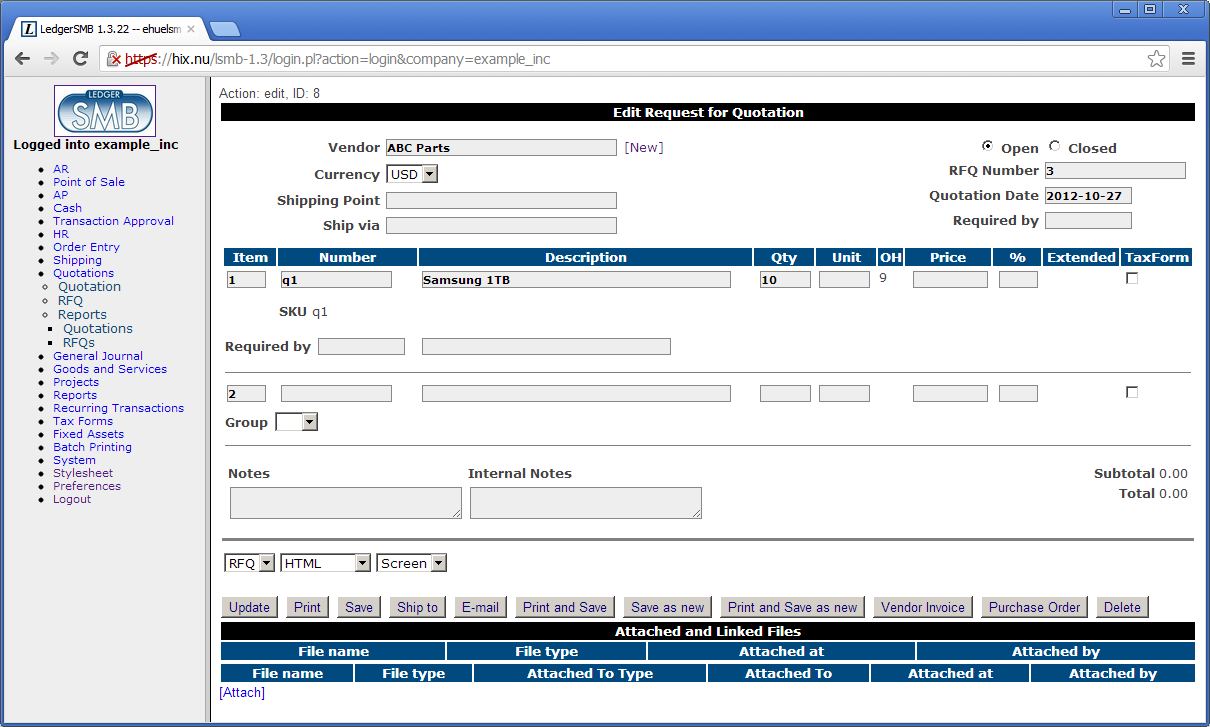
\includegraphics[width=7cm]{rfq-edit-screen.png}
\caption{RFQ entry screen}
\label{fig:bus-rfq-edit-screen}
\end{figure}

Jack clicks the ``Purchase Order'' button which creates a new order from the data in the RFQ.
He completes it
by entering the prices his vendor has quoted and by modifying it to be in accordance with the
quotation. See \secref{sec:QuotationsFromOrders} for more
detail on the order entry screen. When finished he saves the order and mails it to
ABC Parts just like he mailed the \gls{rfq} in the previous section.

\figref{fig:purchase-order-screen} shows the screen of a saved purchase order.

\section{Receiving ordered items}




\section{Receiving an invoice}

\section{Paying an invoice}


\chapter{Ramping up to the first sale}
\label{cha:ramping-up-to-the-first-sale}

% sending out a quote followed by a sales order

\chapter{Shipping sales}
\label{cha:shipping-sales}

\chapter{Invoicing}
\label{cha:invoicing}

\section{Handling sales taxes}

% invoices with taxes included

% invoices with explicit tax amounts

% 


\chapter{Collecting sales invoice payments}
\label{cha:customer-payments}

\section{Customer payments}

\section{Customer payment mismatch}

% choosing between pardonning and registering underpayment

% large ones, as in partial payments or largish under/over payments

% pardonning small mismatches


\chapter{Paying vendor invoices}
\label{cha:vendor-payments}

% handling vendors who match amounts to exact invoices

% handling vendors with running balances

% handling bounced checks: voiding checks to undo payments of vendor invoices
%   relating to bounced checks

\chapter{Monitoring arrears}
\label{cha:monitoring-arrears}

% handling interest on arrears

\chapter{Branching out: services}

% including creation / assignment to different accounts


\section{Recording service hours}

\section{Customer approval on service hours}

\section{Invoicing services}

\chapter{Branching out II: service subscriptions}


